\documentclass[14pt]{extbook}
\usepackage{multicol, enumerate, enumitem, hyperref, color, soul, setspace, parskip, fancyhdr} %General Packages
\usepackage{amssymb, amsthm, amsmath, latexsym, units, mathtools} %Math Packages
\everymath{\displaystyle} %All math in Display Style
% Packages with additional options
\usepackage[headsep=0.5cm,headheight=12pt, left=1 in,right= 1 in,top= 1 in,bottom= 1 in]{geometry}
\usepackage[usenames,dvipsnames]{xcolor}
\usepackage{dashrule}  % Package to use the command below to create lines between items
\newcommand{\litem}[1]{\item#1\hspace*{-1cm}\rule{\textwidth}{0.4pt}}
\pagestyle{fancy}
\lhead{Progress Quiz 10}
\chead{}
\rhead{Version A}
\lfoot{1995-1928}
\cfoot{}
\rfoot{test}
\begin{document}

\begin{enumerate}
\litem{
Graph the equation below.\[ f(x) = (x+1)^2 - 20 \]\begin{enumerate}[label=\Alph*.]
\begin{multicols}{2}\item 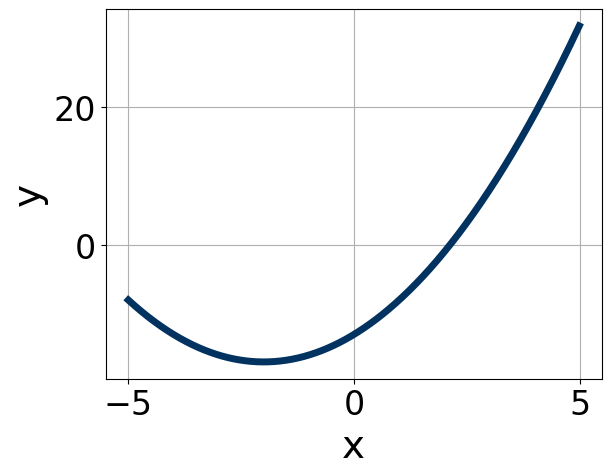
\includegraphics[width = 0.3\textwidth]{../Figures/quadraticEquationToGraphCopyAA.png}\item 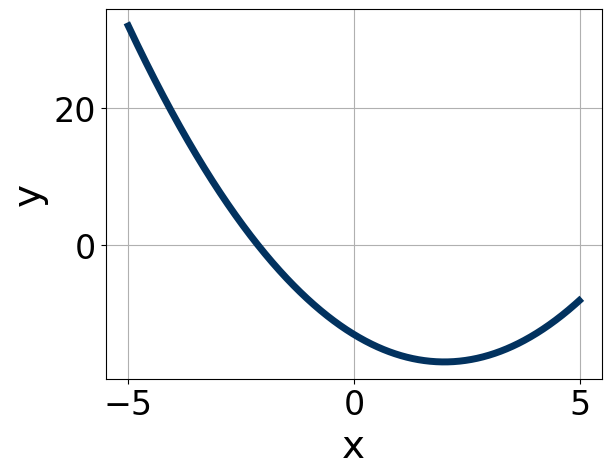
\includegraphics[width = 0.3\textwidth]{../Figures/quadraticEquationToGraphCopyBA.png}\item 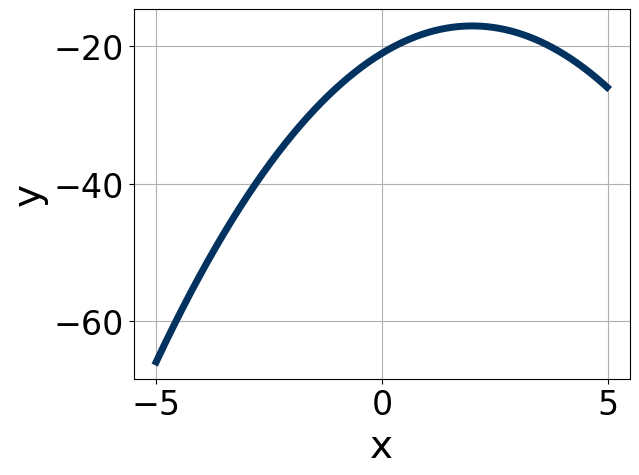
\includegraphics[width = 0.3\textwidth]{../Figures/quadraticEquationToGraphCopyCA.png}\item 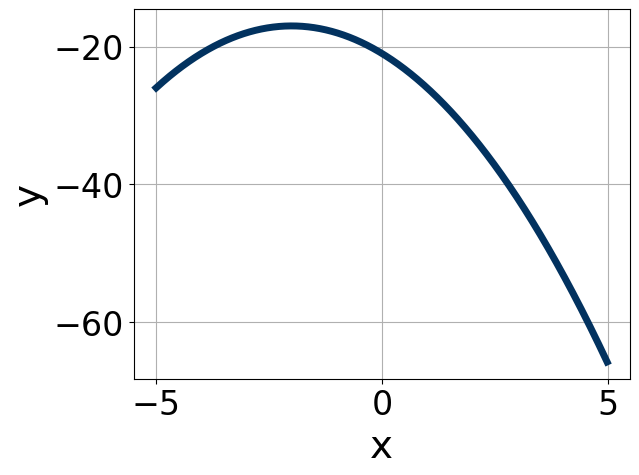
\includegraphics[width = 0.3\textwidth]{../Figures/quadraticEquationToGraphCopyDA.png}\end{multicols}\item None of the above.
\end{enumerate} }
\litem{
Solve the quadratic equation below. Then, choose the intervals that the solutions belong to, with $x_1 \leq x_2$ (if they exist).\[ -19x^{2} +11 x + 7 = 0 \]\begin{enumerate}[label=\Alph*.]
\item \( x_1 \in [-0.9, 0.1] \text{ and } x_2 \in [0.64, 1.06] \)
\item \( x_1 \in [-20.3, -17.7] \text{ and } x_2 \in [6.99, 7.51] \)
\item \( x_1 \in [-2.2, -0.9] \text{ and } x_2 \in [-0.02, 0.46] \)
\item \( x_1 \in [-26.7, -22.7] \text{ and } x_2 \in [25.79, 25.87] \)
\item \( \text{There are no Real solutions.} \)

\end{enumerate} }
\litem{
Factor the quadratic below. Then, choose the intervals that contain the constants in the form $(ax+b)(cx+d); b \leq d.$\[ 36x^{2} +60 x + 25 \]\begin{enumerate}[label=\Alph*.]
\item \( a \in [3.6, 6.2], \hspace*{5mm} b \in [1, 11], \hspace*{5mm} c \in [5.88, 6.6], \text{ and } \hspace*{5mm} d \in [2, 7] \)
\item \( a \in [0.8, 1.8], \hspace*{5mm} b \in [30, 35], \hspace*{5mm} c \in [0.21, 1.16], \text{ and } \hspace*{5mm} d \in [28, 33] \)
\item \( a \in [16.6, 18.5], \hspace*{5mm} b \in [1, 11], \hspace*{5mm} c \in [1.34, 2.33], \text{ and } \hspace*{5mm} d \in [2, 7] \)
\item \( a \in [1.7, 2.1], \hspace*{5mm} b \in [1, 11], \hspace*{5mm} c \in [17.99, 18.26], \text{ and } \hspace*{5mm} d \in [2, 7] \)
\item \( \text{None of the above.} \)

\end{enumerate} }
\litem{
Write the equation of the graph presented below in the form $f(x)=ax^2+bx+c$, assuming  $a=1$ or $a=-1$. Then, choose the intervals that $a, b,$ and $c$ belong to.
\begin{center}
    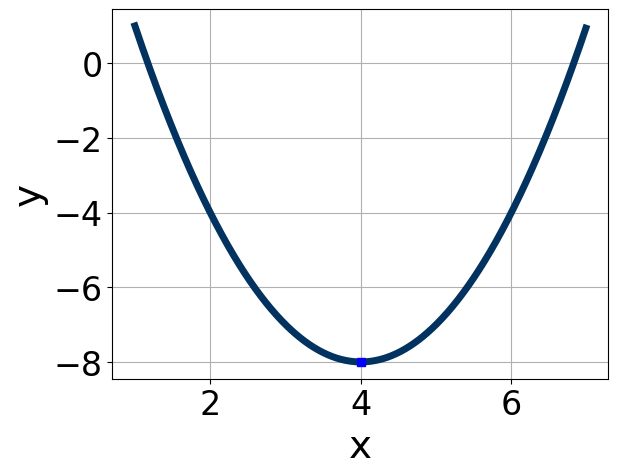
\includegraphics[width=0.5\textwidth]{../Figures/quadraticGraphToEquationCopyA.png}
\end{center}
\begin{enumerate}[label=\Alph*.]
\item \( a \in [0, 3], \hspace*{5mm} b \in [-10, -5], \text{ and } \hspace*{5mm} c \in [10, 15] \)
\item \( a \in [-4, 0], \hspace*{5mm} b \in [-10, -5], \text{ and } \hspace*{5mm} c \in [-20, -17] \)
\item \( a \in [0, 3], \hspace*{5mm} b \in [6, 10], \text{ and } \hspace*{5mm} c \in [10, 15] \)
\item \( a \in [0, 3], \hspace*{5mm} b \in [-10, -5], \text{ and } \hspace*{5mm} c \in [18, 20] \)
\item \( a \in [-4, 0], \hspace*{5mm} b \in [6, 10], \text{ and } \hspace*{5mm} c \in [-20, -17] \)

\end{enumerate} }
\litem{
Solve the quadratic equation below. Then, choose the intervals that the solutions $x_1$ and $x_2$ belong to, with $x_1 \leq x_2$.\[ 15x^{2} -47 x + 36 = 0 \]\begin{enumerate}[label=\Alph*.]
\item \( x_1 \in [1.12, 1.37] \text{ and } x_2 \in [1.72, 2.55] \)
\item \( x_1 \in [0.5, 0.63] \text{ and } x_2 \in [3.9, 4] \)
\item \( x_1 \in [0.42, 0.54] \text{ and } x_2 \in [5.36, 5.55] \)
\item \( x_1 \in [19.8, 20.1] \text{ and } x_2 \in [26.38, 27.31] \)
\item \( x_1 \in [0.76, 1] \text{ and } x_2 \in [2.48, 2.73] \)

\end{enumerate} }
\litem{
Factor the quadratic below. Then, choose the intervals that contain the constants in the form $(ax+b)(cx+d); b \leq d.$\[ 36x^{2} -60 x + 25 \]\begin{enumerate}[label=\Alph*.]
\item \( a \in [11.7, 14.4], \hspace*{5mm} b \in [-11, -4], \hspace*{5mm} c \in [2.4, 3.2], \text{ and } \hspace*{5mm} d \in [-9, -2] \)
\item \( a \in [1.9, 3.9], \hspace*{5mm} b \in [-11, -4], \hspace*{5mm} c \in [17.8, 19.6], \text{ and } \hspace*{5mm} d \in [-9, -2] \)
\item \( a \in [5.6, 8.4], \hspace*{5mm} b \in [-11, -4], \hspace*{5mm} c \in [4.9, 7.3], \text{ and } \hspace*{5mm} d \in [-9, -2] \)
\item \( a \in [0.5, 1.5], \hspace*{5mm} b \in [-31, -26], \hspace*{5mm} c \in [-0.7, 1.6], \text{ and } \hspace*{5mm} d \in [-30, -26] \)
\item \( \text{None of the above.} \)

\end{enumerate} }
\litem{
Solve the quadratic equation below. Then, choose the intervals that the solutions belong to, with $x_1 \leq x_2$ (if they exist).\[ 14x^{2} +9 x -3 = 0 \]\begin{enumerate}[label=\Alph*.]
\item \( x_1 \in [-1.97, -0.26] \text{ and } x_2 \in [-0.1, 0.8] \)
\item \( x_1 \in [-12.81, -12.15] \text{ and } x_2 \in [1.8, 4.1] \)
\item \( x_1 \in [-0.38, -0.11] \text{ and } x_2 \in [0.3, 2.1] \)
\item \( x_1 \in [-16.76, -15.75] \text{ and } x_2 \in [15.2, 16.8] \)
\item \( \text{There are no Real solutions.} \)

\end{enumerate} }
\litem{
Solve the quadratic equation below. Then, choose the intervals that the solutions $x_1$ and $x_2$ belong to, with $x_1 \leq x_2$.\[ 12x^{2} +43 x + 36 = 0 \]\begin{enumerate}[label=\Alph*.]
\item \( x_1 \in [-27.88, -26.97] \text{ and } x_2 \in [-16.12, -15.86] \)
\item \( x_1 \in [-2.28, -1.8] \text{ and } x_2 \in [-1.43, -1.26] \)
\item \( x_1 \in [-3.29, -2.58] \text{ and } x_2 \in [-1.31, -0.94] \)
\item \( x_1 \in [-6.8, -5.55] \text{ and } x_2 \in [-0.45, -0.43] \)
\item \( x_1 \in [-9.3, -8.79] \text{ and } x_2 \in [-0.36, -0.18] \)

\end{enumerate} }
\litem{
Write the equation of the graph presented below in the form $f(x)=ax^2+bx+c$, assuming  $a=1$ or $a=-1$. Then, choose the intervals that $a, b,$ and $c$ belong to.
\begin{center}
    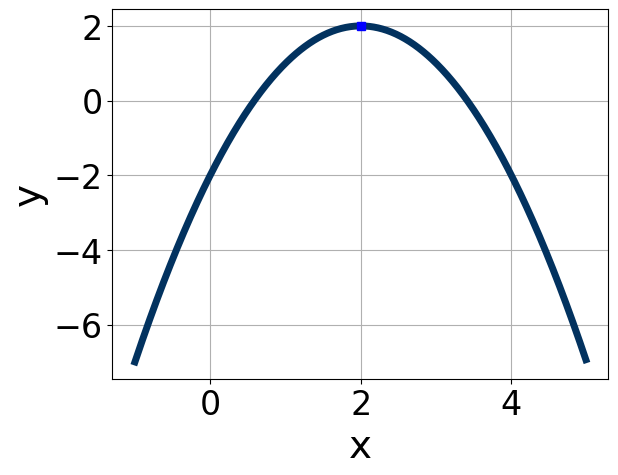
\includegraphics[width=0.5\textwidth]{../Figures/quadraticGraphToEquationA.png}
\end{center}
\begin{enumerate}[label=\Alph*.]
\item \( a \in [-1.8, -0.7], \hspace*{5mm} b \in [4, 6], \text{ and } \hspace*{5mm} c \in [-2, 1] \)
\item \( a \in [-1.8, -0.7], \hspace*{5mm} b \in [-7, 1], \text{ and } \hspace*{5mm} c \in [-2, 1] \)
\item \( a \in [-0.6, 1.6], \hspace*{5mm} b \in [4, 6], \text{ and } \hspace*{5mm} c \in [2, 8] \)
\item \( a \in [-1.8, -0.7], \hspace*{5mm} b \in [-7, 1], \text{ and } \hspace*{5mm} c \in [-7, -5] \)
\item \( a \in [-0.6, 1.6], \hspace*{5mm} b \in [-7, 1], \text{ and } \hspace*{5mm} c \in [2, 8] \)

\end{enumerate} }
\litem{
Graph the equation below.\[ f(x) = (x+2)^2 - 20 \]\begin{enumerate}[label=\Alph*.]
\begin{multicols}{2}\item 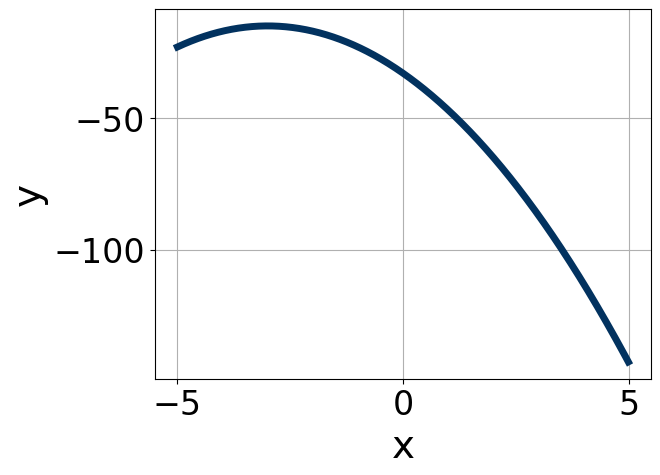
\includegraphics[width = 0.3\textwidth]{../Figures/quadraticEquationToGraphAA.png}\item 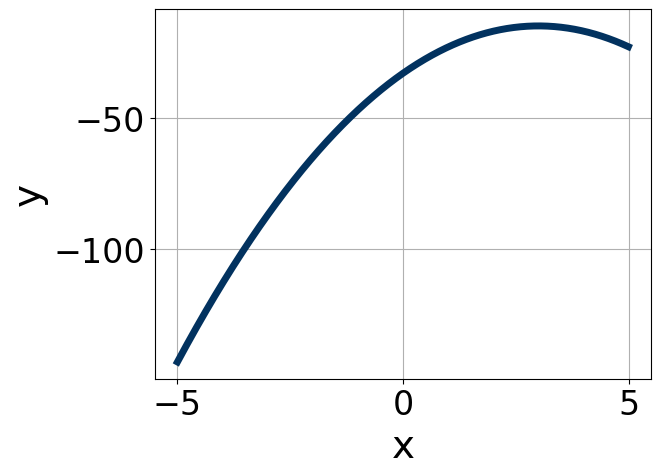
\includegraphics[width = 0.3\textwidth]{../Figures/quadraticEquationToGraphBA.png}\item 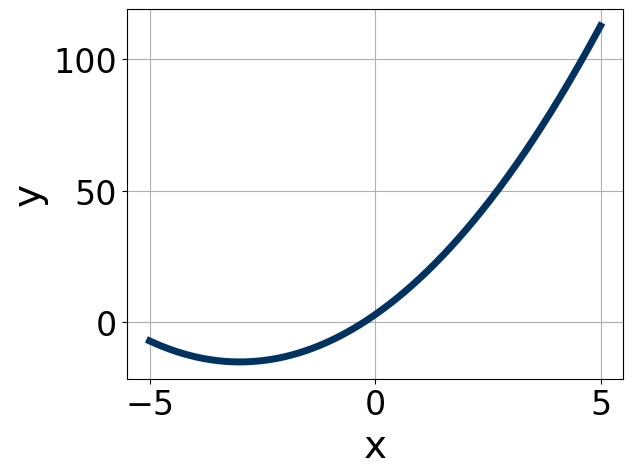
\includegraphics[width = 0.3\textwidth]{../Figures/quadraticEquationToGraphCA.png}\item 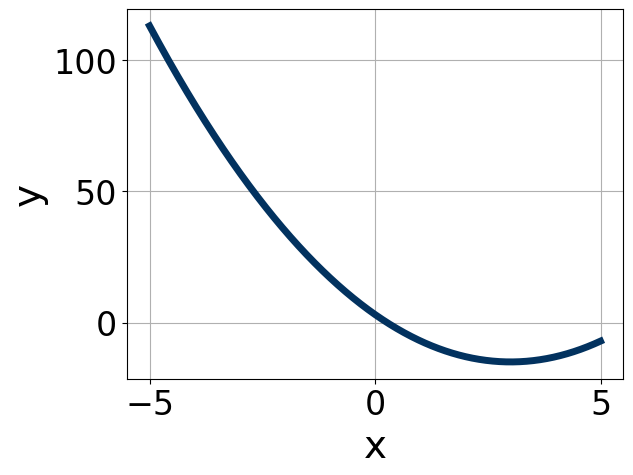
\includegraphics[width = 0.3\textwidth]{../Figures/quadraticEquationToGraphDA.png}\end{multicols}\item None of the above.
\end{enumerate} }
\end{enumerate}

\end{document}